\section{Results}
\label{sec:results}

\subsection{AIMSpice}

The register could have different effect and operations due to the corner of the transistor and the temperature. There are five corners the transistors could be; TT(typical-typical), SS(slow-slow), FF(fast-fast), SF(slow-fast) and FS(fast-slow).  For all of the corners they have been tested for three temperatures, 0 $^\circ$C, 27 $^\circ$C and 70 $^\circ$C. All the different plots for the different cases are shown in \autoref{appendix:register_plots}. 

To validate the functionality of the register, one can examine the plot of the TT corner at 27$^\circ C$. 

\begin{figure}[H]
    \centering
    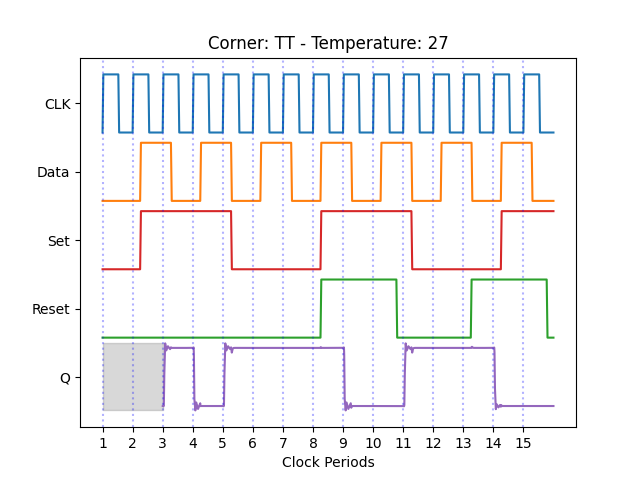
\includegraphics[width=0.9\textwidth]{Figures/Aimspice_Plots/TT_27.png}
    \caption{Plot of register for TT corner.}
    \label{fig:result_TT27}
\end{figure}

As shown in \autoref{fig:result_TT27}, the different combinations of the inputs signals gives the expected Q-value based on \autoref{tab:registerFunc}. If the Set-value is high, Q only updates to the D-value when the CLK changes from low to high. And if the Reset-value is high, the value Q is overruled to low, even if Set and D is high. This is also the case for the other temperatures and corners in \autoref{appendix:register_plots}.

The stability of the register, when changing from low to high, is affected by different corners or operating temperatures. \autoref{fig:TT_diffTemps} and \autoref{fig:27_diffCorners} shows the stability for the same corner with different temperatures and different corners at same temperature respectively. The other plots for the different corners and temperatures can be found in \autoref{appendix:register_stability}.

\begin{figure}[H]
    \begin{minipage}{0.5\textwidth}
        \centering
        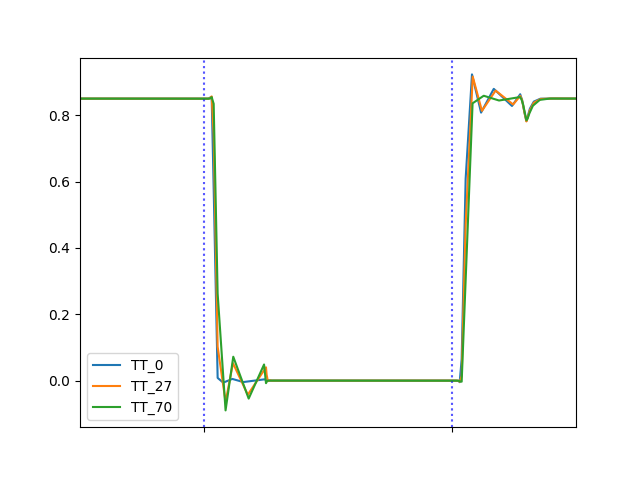
\includegraphics[width=\textwidth]{Figures/Aimspice_Plots/CornerTT.png}
        \caption{\parbox{0.5\textwidth}{Plot of changes in Q-value with TT corner at different temperatures.}}
        \label{fig:TT_diffTemps}
    \end{minipage}%
    \begin{minipage}{0.5\textwidth}
        \centering
        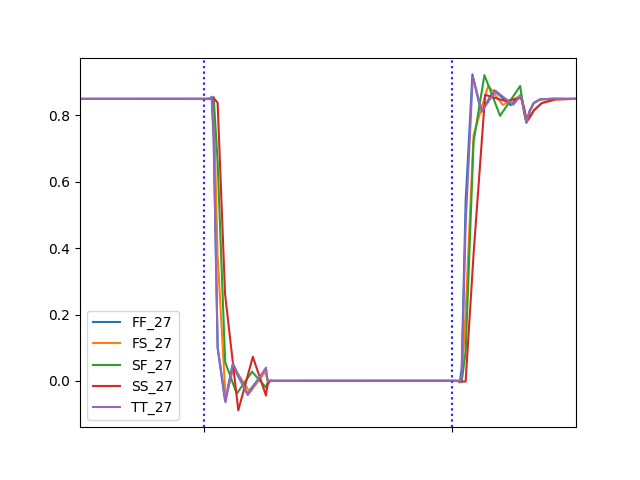
\includegraphics[width=\textwidth]{Figures/Aimspice_Plots/Temperatur27.png}
        \caption{\parbox{0.4\textwidth}{Plot of changes in Q-value with the different corners at 27 $^\circ$C}}
        \label{fig:27_diffCorners}
    \end{minipage}
\end{figure}

\subsubsection{Static Power Consumption}

As mentioned in \autoref{subsubsec:SPC_Calc}, a low voltage on $V_{DD}$ is optimal. We have therefore chosen a value for $V_{DD} = 0.85$ V, since that fulfills the specification 12 in \autoref{tab:specifications}. This value of $V_{DD}$ was chosen as through testing we found that a lower voltage would result in unstable functionality. By using the function operating point in AIMSpice, the leakage current in the $V_{DD}$ node can be found.

\autoref{tab:leakage} shows the different leakage currents for the TT and FF corners with all three temperatures. To calculate the static power consumption, we use the \autoref{eq:power} for all the values and get  \autoref{tab:power}.

\begin{table}[H]
\centering
\caption{Leakage Current.}
\label{tab:leakage}
\resizebox{0.4\columnwidth}{!}{%
    \begin{tabular}{lll}
    \cline{2-3}
    \multicolumn{1}{l|}{} &
      \multicolumn{1}{l|}{\cellcolor[HTML]{C0C0C0}TT} &
      \multicolumn{1}{l|}{\cellcolor[HTML]{C0C0C0}FF} \\ \hline
    \multicolumn{1}{|l|}{\cellcolor[HTML]{C0C0C0}0 $^\circ$C} &
      \multicolumn{1}{l|}{1.0931 nA} &
      \multicolumn{1}{l|}{3.1854 nA} \\ \hline
    \multicolumn{1}{|l|}{\cellcolor[HTML]{C0C0C0}27 $^\circ$C} &
      \multicolumn{1}{l|}{3.0325 nA} &
      \multicolumn{1}{l|}{8.5711 nA} \\ \hline
    \multicolumn{1}{|l|}{\cellcolor[HTML]{C0C0C0}70 $^\circ$C} &
      \multicolumn{1}{l|}{6.9843 nA} &
      \multicolumn{1}{l|}{13.513 nA} \\ \hline
     &  &  
    \end{tabular}%
}
\end{table}

\begin{table}[H]
\centering
\caption{Static Power Consumption.}
\label{tab:power}
\resizebox{0.4\columnwidth}{!}{%
\begin{tabular}{lll}
\cline{2-3}
\multicolumn{1}{l|}{} &
  \multicolumn{1}{l|}{\cellcolor[HTML]{C0C0C0}TT} &
  \multicolumn{1}{l|}{\cellcolor[HTML]{C0C0C0}FF} \\ \hline
\multicolumn{1}{|l|}{\cellcolor[HTML]{C0C0C0}0 $^\circ$C} &
  \multicolumn{1}{l|}{0.92914 nW} &
  \multicolumn{1}{l|}{2.7076 nW} \\ \hline
\multicolumn{1}{|l|}{\cellcolor[HTML]{C0C0C0}27 $^\circ$C} &
  \multicolumn{1}{l|}{2.5776 nW} &
  \multicolumn{1}{l|}{7.2854 nW} \\ \hline
\multicolumn{1}{|l|}{\cellcolor[HTML]{C0C0C0}70 $^\circ$C} &
  \multicolumn{1}{l|}{5.9367 nW} &
  \multicolumn{1}{l|}{11.486 nW} \\ \hline
 &  &  
\end{tabular}
}
\end{table}

\subsection{Verilog Testbench Results}

In this subsection, results of Verilog-simulations is presented. All Verilog-code is given in \autoref{appendix:Verilog-code} and \ref{sec:verilog_testbenches}.

\subsubsection{FSM Results}
\label{subsubsec:fsm_results}

\noindent
The timing diagram generated by the FSM testbench is shown in \autoref{fig:fsm_simulation}. The timing diagram includes the input signals CLK and I[1:0], the output signal CTRL[1:0] (shown as O[1:0] in the figure) and the current state C[1:0], which is an internal value in the FSM. For simplicity, values for I and O are shown in binary notation and values for C are shown in decimal notation.

\begin{figure}[H]
    \centering
    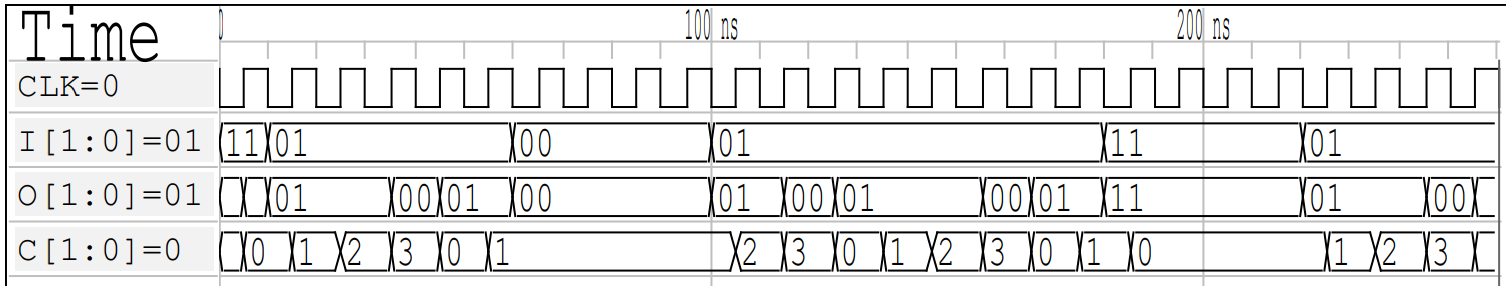
\includegraphics[width=\textwidth]{Figures/FSM_testbench_out.png}
    \caption{Timing diagram of FSM simulated in Verilog.}
    \label{fig:fsm_simulation}
\end{figure}

The diagram shows the state register being reset on the first rising edge of the CLK. As the input changes to ``01'', the FSM cycles through the states 0, 1, 2, and 3. The first three states, 0, 1, and 2, output the control signals ``01'' meaning ``run a mac operation'', while state 3 outputs ``00'', meaning ``pause the MAC and hold the stored value''. When the input is ``00'', the FSM pauses on its current state before continuing when the input returns to ``01''. When the input is ``11'', the state is forced to 0 and the output is ``11'' which should reset the accumulator in the MAC.

\subsubsection{MAC Results}
\label{subsubsec:mac_results}

The output provided by the multiplier testbench is shown in \autoref{fig:output_multiplier}.

\begin{figure}[H]
\centering

\begin{minipage}{0.8\textwidth}
\begin{lstlisting}[style=outputstyle]
[Running] Multiplier_Testbench.v
VCD info: dumpfile Multiplier_Testbench.vcd opened for output.
0*0= 0

[...]

3*3= 9
No errors found
Multiplier_Testbench.v:34: $finish called at 16000 (1ps)
[Done] exit with code=0 in 0.522 seconds
\end{lstlisting}
\end{minipage}
\caption{Output from the Multiplier Testbench.}
\label{fig:output_multiplier}
\end{figure}

\noindent
The output provided by the adder testbench is shown in \autoref{fig:output_adder}.

\begin{figure}[H]
\centering
\begin{minipage}{0.8\textwidth}
\begin{lstlisting}[style=outputstyle]
[Running] Adder_Testbench.v
VCD info: dumpfile Adder_Testbench.vcd opened for output.
  0+  0=  0
  0+  1=  1
  
[...]

255+254=253
255+255=254
Congratulations! No errors found.
Adder_Testbench.v:34: $finish called at 65536000 (1ps)
[Done] exit with code=0 in 1.698 seconds
\end{lstlisting}
\end{minipage}
\caption{Output from the Adder Testbench.}
\label{fig:output_adder}
\end{figure}

\noindent
The output provided by the register testbench is shown in figure \autoref{fig:output_register}.

\begin{figure}[H]
\centering
\begin{minipage}{0.8\textwidth}
\begin{lstlisting}[style=outputstyle]
[Running] Register_Testbench.v
VCD info: dumpfile Register_Testbench.vcd opened for output.
Congratulations! No errors found.
Register_Testbench.v:85: $finish called at 10250000 (1ps)
[Done] exit with code=0 in 0.194 seconds
\end{lstlisting}
\end{minipage}
\caption{Output from the Register Testbench.}
\label{fig:output_register}
\end{figure}

The timing diagram generated by the FSM testbench is shown in \autoref{fig:mac_simulation}. The diagram includes the input signals CLK, A[1:0], B[1:0] and CTRL[1:0] as well as the internal value PROD[3:0] and the output Y[7:0]. PROD[3:0] is an internal value generated by the multiplier, i.e. the product of A and B. For simplicity,
values for CTRL are shown in binary notation, and values for A, B, PROD in decimal notation.

\begin{figure}[H]
    \centering
    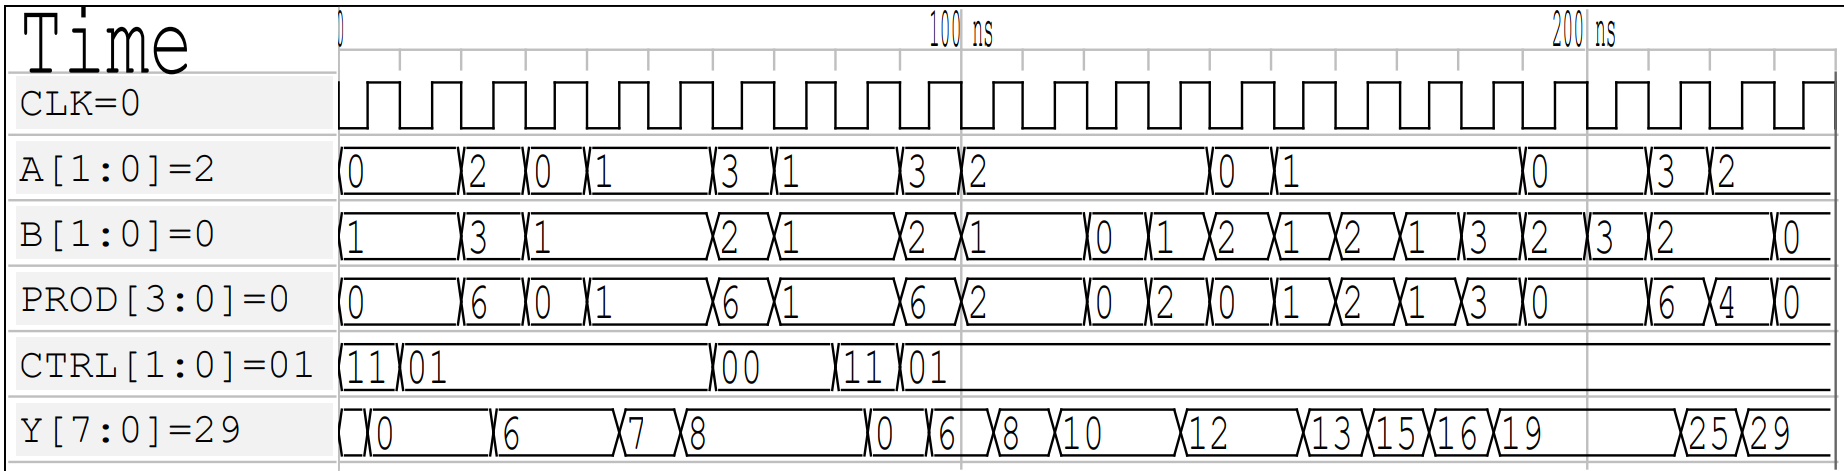
\includegraphics[width=\textwidth]{Figures/Result MAC.png}
    \caption{Timing diagram of MAC simulated in Verilog.}
    \label{fig:mac_simulation}
\end{figure}

The figure shows the 8-bit register initially being reset to 0, before receiving the run control signal ``01''. For each rising CLK edge with this control signal, PROD is added to the previous value of Y. The control signal ``00'' pauses the accumulation and makes the register holds the current value. The control signal 11 resets the register again to 0. 

\subsubsection{Full MAC Results}

The timing diagram generated by the full MAC testbench is shown in \autoref{fig:fullmac_simulation}. The timing diagram includes the input signals CLK, I[1:0], A[1:0], B[1:0], the input signal Y[7:0] as well as the control signal CTRL[1:0] and the intermediate signal PROD[3:0]. For simplicity, all values are shown in decimal notation.

\begin{figure}[H]
    \centering
    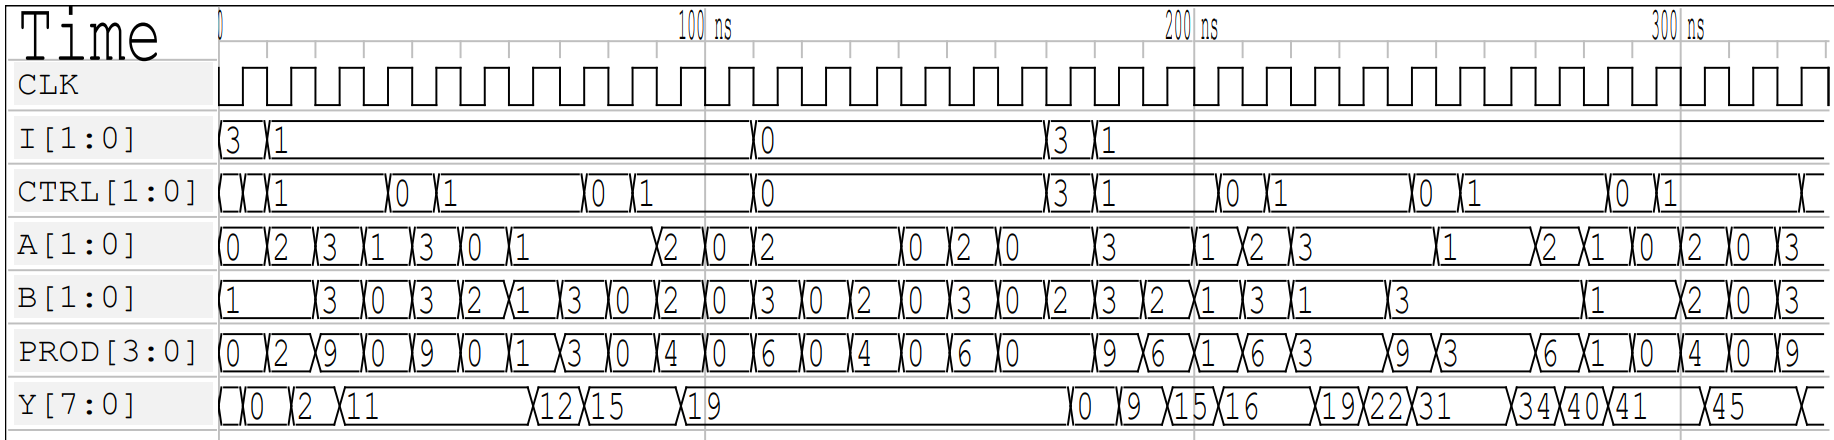
\includegraphics[width=\textwidth]{Figures/Result full MAC3.png}
    \caption{Timing diagram of Full MAC simulated in Verilog.}
    \label{fig:fullmac_simulation}
\end{figure}

Initially, the input signal I[1:0] is ``11'', resetting the state register and the accumulator. As I changes to ``01'', the CTRL-signal holds the 3+1 pattern described in \cite[p.3]{project_description}. The accumulator adds PROD to its output Y for each rising edge while CTRL=01, pausing and holding its value when CTRL=00. At 110 ns, I=00, effectively pausing the MAC-operation at its current value for six CLK-periods. At 170 ns, I=11, which resets the registers in both the FSM and the MAC. From 180 ns the system continues its 3+1 pattern.
